\documentclass{beamer}
\usepackage{graphicx}
\usepackage{amssymb}
\usepackage{perpage}
\usepackage{beamerthemeshadow}

\mode<presentation>
{
  \usetheme{Frankfurt}
}

\setbeamertemplate{footline}[page number]
\usepackage[english]{babel}
\setbeamertemplate{navigation symbols}{}%remove navigation symbols
\newcommand{\bibintext}[1]{{\tiny \bibentry{#1}}}

\usepackage{bibentry}

\def\newblock{\hskip .11em plus .33em minus .07em}
\usepackage{times}

\title[elastic instabilities]{Smoothed dissipative particle dynamics simulations of elastic instabilities in diluted polymer solutions}
\date{}
\nobibliography*

\DeclareGraphicsRule{*}{mps}{*}{}

\author{S. Litvinov, X. Qingguang, M. Ellero, X.Y. Hu and N.A. Adams}

\institute{
  Lehrstuhl f\"{u}r Aerodynamik und Str\"{o}mungsmechanik \\
  TU M\"{u}nich
}

\newcommand{\imgwidth}{0.92\textwidth}
\MakePerPage{footnote} %the perpage package command

\begin{document}
\begin{frame}
  \titlepage
\end{frame}

\begin{frame}
  \tableofcontents
\end{frame}

\section[Motivation]{Motivation}
\begin{frame}
  \frametitle{Motivation: cooling}
  \begin{columns}
    \begin{column}{0.5\textwidth}
      \begin{block}{Why microchannels?}
        \begin{itemize}
        \item Devices are smaller
        \item Higher surface to volume ratio
        \end{itemize}
      \end{block}
      \begin{block}{Why boiling?}
        \begin{itemize}
        \item Heat of evaporation
        \item Uniform and predictable temperature
        \end{itemize}
      \end{block}
    \end{column}
    \begin{column}{0.5\textwidth}
      \begin{figure}
        \centering
        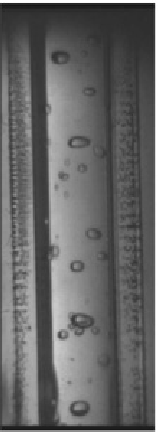
\includegraphics[width=1.1cm]{exp01.png}
        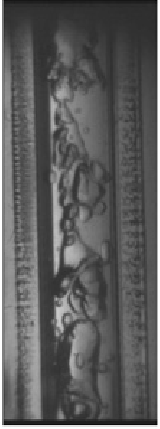
\includegraphics[width=1.1cm]{exp02.png}
        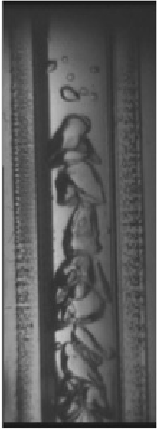
\includegraphics[width=1.1cm]{exp03.png}
        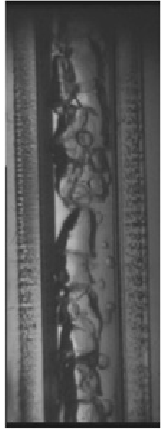
\includegraphics[width=1.1cm]{exp04.png}
        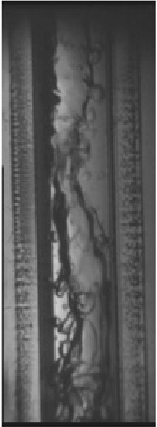
\includegraphics[width=1.1cm]{exp05.png}
        \caption{Flow Boiling Regimes~\footnotemark}
        \label{fig:self}
      \end{figure}
    \end{column}
  \end{columns}
  \footnotetext{\tiny \bibentry{baldassari2012flow}}
\end{frame}

\begin{frame}
  \frametitle{Motivation II}
  \begin{block}{Why microchannels are different?}
    \begin{itemize}
    \item $\Uparrow$ viscosity, diffusion, surface tension, contact lines
    \item $\Downarrow$ gravity, inertia
    \end{itemize}
  \end{block}

  \begin{block}{Viscosity}
    $1<\text{Re}<2000$ $\implies$ full Navier-Stokes (NS) equations~\footnotemark
  \end{block}
  \footnotetext{\tiny \bibentry{worner_numerical_2012}}
\end{frame}

\begin{frame}
  \frametitle{Models}
  \begin{itemize}
  \item VOF \\
    \bibintext{welch_local_1995}, \\
    \bibintext{kunkelmann_cfd_2009}
  \item Lattice Boltzmann \\
    \bibintext{markus_pool_2012}
  \item Particle-Based \\
    \bibintext{muller_particle-based_2005}, \\ 
   \bibintext{yoon_direct_2001}
  \end{itemize}
\end{frame}

\section[Model]{Model}
\begin{frame}
  \frametitle{Parts of the model}
  \begin{itemize}
  \item Navier-Stokes equations for velocity
  \item Surface tension forces on the interface~\footnotemark
  \item \alert{Heat conduction~\footnotemark[2]}
  \item \alert{Evaporation model}
  \end{itemize}
  \begin{block}{Assumption}
    Evaporation rate is controlled by heat supply
    $\Longleftrightarrow$ vapor contains as little energy as it can
    without condensation $\Longleftrightarrow$ vapor is at $T=T_s$
  \end{block}

  \footnotetext{\tiny \bibentry{Hu2006}}
  \footnotetext[2]{\tiny \bibentry{Cleary1999}}
\end{frame}

\begin{frame}
  \frametitle{Heat conduction}
  \begin{equation}
    \label{eq:heatConductionTerm}
    \frac{\partial U_i}{\partial t} = \sum_j\frac{4 m_i}{\rho_j \rho_i} \frac{k_j k_i}{k_j + k_i} \alert{T_{ij}} \frac{\partial W}{\partial r_{ij}}
  \end{equation}
  \begin{equation}
    \label{eq:ideal}
    U_i = c_{v,i} T_i
  \end{equation}
  For vapor-vapor and liquid-liquid interaction:
  \begin{equation}
    \label{eq:tij}
    T_{ij} = \frac{2T_i \alert{T_j}}{T_i + \alert{T_j}}
  \end{equation}
  For liquid-vapor
  \begin{equation}
    \label{eq:tab}
    T_{ij} = \frac{2T_i \alert{T_s}}{T_i + \alert{T_s}}
  \end{equation}
  where $T_s$ is a saturation temperature
\end{frame}

\begin{frame}
  \frametitle{Evaporation model: particle creation}
  \begin{block}{Rule}
    If a vapor particle has $T>T_s$ and has a liquid particle as a
    neighbor we create a new vapor particle
  \end{block}
  \begin{itemize}
  \item mass is from a liquid particle ($m_{liquid} >> m_{vapor}$)
  \item energy goes to vapor particle
  \item mechanical momentum is distributed between ``new'' and ``old''
    vapor particles
  \end{itemize}
\end{frame}

\section{Validation}
\begin{frame}
  \frametitle{A bubble growth}
  \begin{itemize}
  \item Initial condition: ``seed'' vapor particles in the center of
    the domain
  \item Domain is periodic, edges of the domain $T=T_s +
    \Delta T$
  \item Theory predicts a self similar temperature profile $T =
    T(r/R(t))$, where $r$~---~distance from the center, $R(t)$~---~radius of
    the bubble
  \end{itemize}
\end{frame}

\begin{frame}
  \frametitle{A bubble growth}
  \begin{figure}
    \centering
    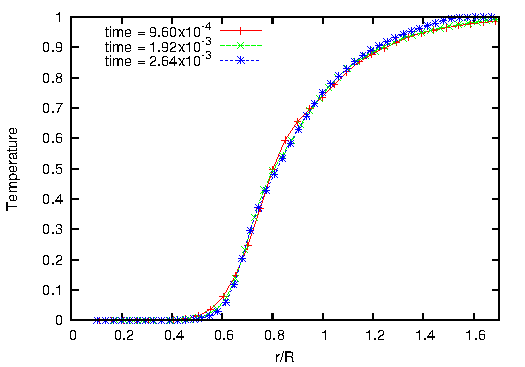
\includegraphics{gnuplot/self.pdf}
    \caption{Temperature profile at different times vs normalized
      distance from the center of the domain}
    \label{fig:self}
  \end{figure}
\end{frame}

\begin{frame}
  \frametitle{A bubble growth}
  \begin{figure}[ht]
    \centering
    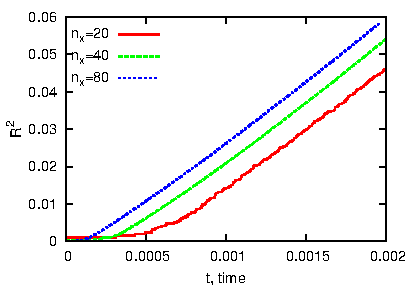
\includegraphics{gnuplot/f1.pdf}
    \caption{Radius of the bubble vs time. Theory: $R(t) \propto \sqrt{t}$}
    \label{fig:dep}
  \end{figure}
\end{frame}

\begin{frame}
  \frametitle{Departure of the bubble from the wall}
  \begin{itemize}
  \item Bottom and top: wall, rest of the boundaries are periodic
  \item Initial condition: the bottom wall temperature $T=T_s + \Delta T$
  \item Initial condition: the bulk temperature $T=T_s$
  \item ``Seed'' vapor particles at the center of the bottom wall
  \item Buoyancy vs surface tension
  \end{itemize}
\end{frame}

\begin{frame}
  \frametitle{Departure of the bubble from the wall}
  \begin{figure}[ht]
    \centering
    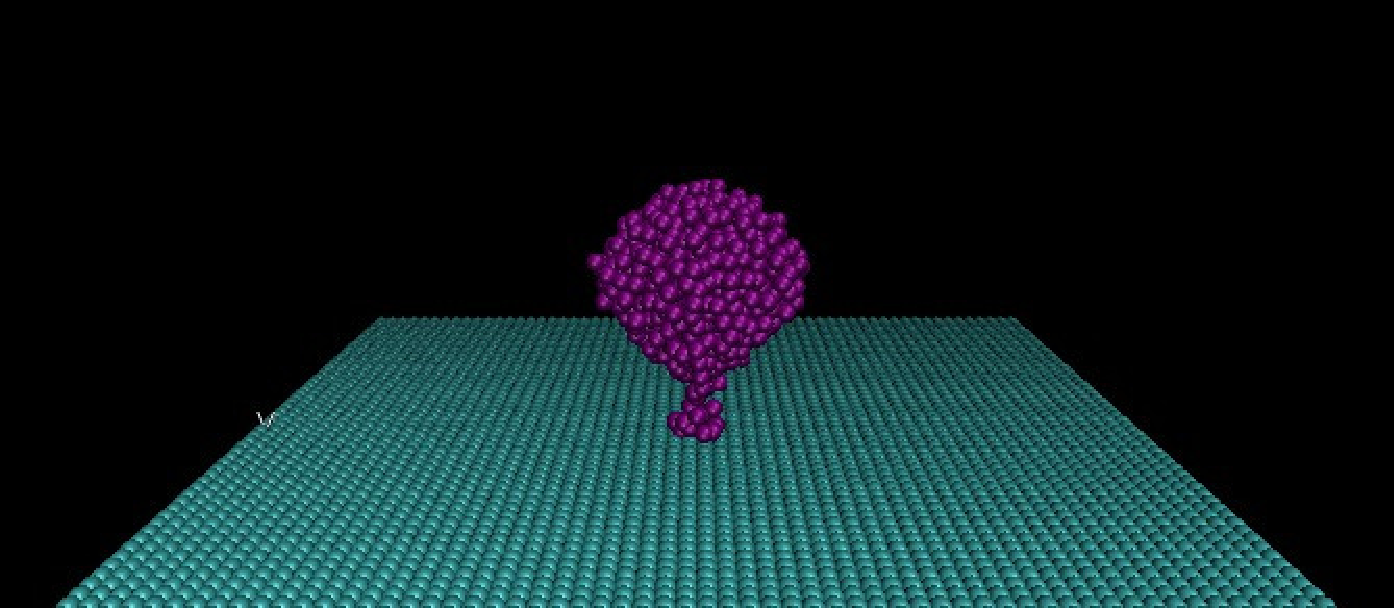
\includegraphics[width=0.8\textwidth]{gnuplot/dep-59.pdf}
    \caption{Snapshot of bubble departure from the super-heated
      surface. Liquid particles are not shown.}
    \label{fig:snapshot}
  \end{figure}
\end{frame}

\begin{frame}
  \begin{figure}[t]
    \centering
    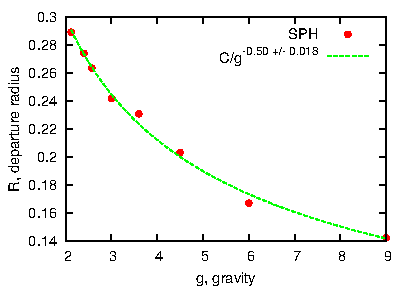
\includegraphics{gnuplot/dep.pdf}
    \caption{Bubble departure radios versus gravity
      force. Theory:~$R_{dep} \propto 1/\sqrt{g})$ }
    \label{fig:radii}
  \end{figure}
  \bibliographystyle{elsart-num}
  \nobibliography{bibdata,intro}
\end{frame}

\section{Conclusions}
\begin{frame}
  \frametitle{Conclusions}
  \begin{itemize}
  \item Particle based model for evaporation is proposed
  \item Heat supply is a rate limiting step: superheated and subheated
    liquid
  \item Model is tested for bubble growth and bubble departure
  \end{itemize}
\end{frame}
\end{document}
